\setlength{\parskip}{\baselineskip}
\section{Results}

\begin{frame}
	\huge Results
\end{frame}

\begin{frame}{Compared Platforms: CPU}
	\center{\large{Intel i7 4710MQ}}
	\begin{table}[H]
		\centering
		\begin{tabular}{ll}
			\toprule
			\textbf{Cores / Threads}      & 4/8      \\
			\textbf{Max Turbo Frequency}  & 3.5GHz   \\
			\textbf{TDP}                  & 47W      \\
			\textbf{Max Memory Bandwidth} & 25.6GB/s \\
			\textbf{Lithography}          & 22nm     \\
			\bottomrule
		\end{tabular}
	\end{table}
\end{frame}

\begin{frame}{Compared Platforms: GPU}
	\center{\large{NVIDIA RTX-2060 Super 8GB}}
	\begin{table}[H]
		\centering
		\begin{tabular}{ll}
			\toprule
			\textbf{CUDA Cores}        & 2176      \\
			\textbf{Tensor Cores}      & 32        \\
			\textbf{GPU Memory}        & 8GB GDDR6 \\
			\textbf{Boost Clock}       & 1650 MHz  \\
			\textbf{Memory Interface}  & 256-bit   \\
			\textbf{Memory Bandwidth}  & 448GB/s   \\
			\textbf{Power Consumption} & 175W      \\
			\bottomrule
		\end{tabular}
	\end{table}
\end{frame}

\begin{frame}{Compared Platforms: FPGA}
	\center{\large{Xilinx CHaiDNN}}
	\begin{table}[H]
		\centering
		\begin{tabular}{ll}
			\toprule
			\textbf{PL/DSP Clock Frequency} & 250/500 MHz \\
			\textbf{LUT Usage}              & 59.1\%      \\
			% 		\textbf{LUTRAM Usage} & -\\
			\textbf{FF Usage}               & 27.66\%     \\
			\textbf{BRAM Usage}             & 74.12\%     \\
			\textbf{DSP Usage}              & 53.65\%     \\
			% 		\textbf{BUFG Usage} & -\\
			\bottomrule
		\end{tabular}
	\end{table}
\end{frame}

\begin{frame}{Compared Platforms: FPGA}
	\center{\large{Proposed Platform}}
	\begin{table}[H]
		\centering
		\begin{tabular}{ll}
			\toprule
			\textbf{Clock Frequency (MHz)} & 300MHz \\
			\textbf{LUT Usage}             & 7.34\% \\
			\textbf{LUTRAM Usage}          & 2.05\% \\
			\textbf{FF Usage}              & 4.03\% \\
			\textbf{BRAM Usage}            & 7.51\% \\
			\textbf{DSP Usage}             & 1.9\%  \\
			% \textbf{BUFG (\%)}             & 0.25\% \\
			\bottomrule
		\end{tabular}
	\end{table}
\end{frame}

\begin{frame}{CPU \& GPU Performance}
	\begin{itemize}
		\item Inference 2500 images
		\item Use all worker \& batch-size combinations
		\item PyTorch pre-built pre-trained AlexNet
	\end{itemize}
\end{frame}

\begin{frame}{CPU \& GPU Performance: Latency}
	\centering
	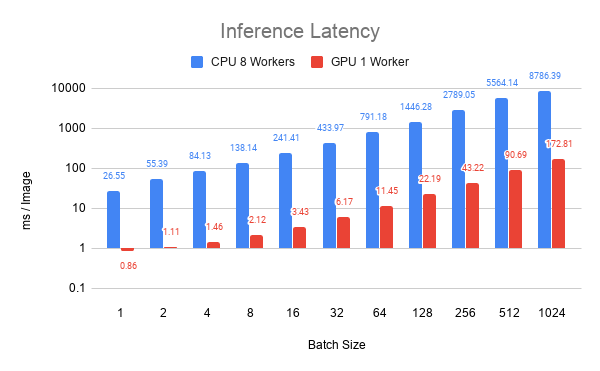
\includegraphics[width=0.7\textwidth]{../Images/Results/CPU-GPU-Inference-Latency.png}\\
\end{frame}

\begin{frame}{CPU \& GPU Performance: Throughput}
	\centering
	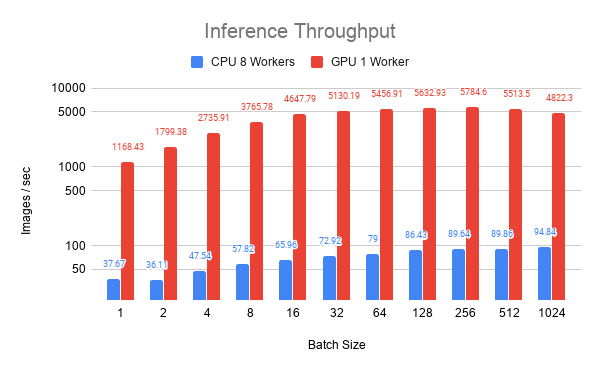
\includegraphics[width=0.7\textwidth]{../Images/Results/CPU-GPU-Inference-Throughput.png}\\
\end{frame}

\begin{frame}{Final Performance}
	\begin{table}[H]
		\centering
		\begin{tabular}{l|l|l|l|l}
			\toprule
			                                    & \textbf{CPU} & \textbf{GPU} & \textbf{CHaiDNN} & \textbf{Proposed Platform} \\
			\midrule
			\textbf{Clock Frequency (MHz)}      & 3500         & 1650         & 250/500          & 300                        \\
			\textbf{Throughput (Images/s)}      & 94.84        & 5784.6       & 10.07            & 0.0927                     \\
			\textbf{Throughput Speedup}         & 1x           & 60.9933x     & 0.1062x          & 0.001x                     \\
			\textbf{Latency (s)}                & 0.0266       & 0.0009       & 0.0993           & 10.783                     \\
			\textbf{Latency Speedup}            & 1x           & 29.5556x     & 0.2679x          & 0.0025x                    \\
			\textbf{Total On-Chip Power (Watt)} & 47           & 175          & 19.3             & 4.559                      \\
			\textbf{Power Efficiency}           & 1x           & 0.2686x      & 2.4352x          & 10.3093x                   \\
			\textbf{Energy Cons./Image (Joule)} & 1.2502       & 0.1575       & 1.9165           & 49.1597                    \\
			\textbf{Energy Efficiency}          & 1x           & 7.9378x      & 0.6523x          & 0.0254x                    \\
			\textbf{Images/Joule}               & 2.0179       & 33.0549      & 0.5218           & 0.0203                     \\
			\bottomrule
		\end{tabular}
	\end{table}
\end{frame}

\begin{frame}{Final Performance}
	\centering
	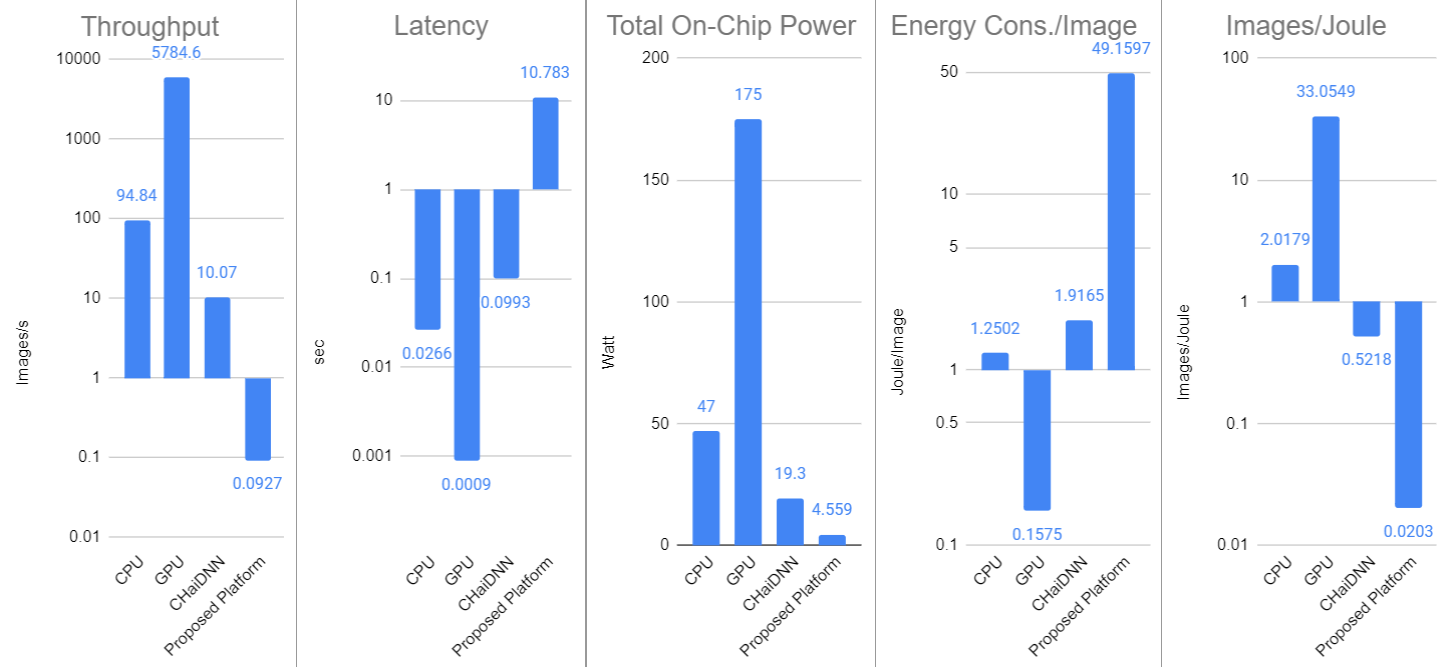
\includegraphics[width=0.9\textwidth]{../Images/Results/Final-Results-charts.png}\\
\end{frame}
